
\section{Redes Complexas}
\label{section:metodologia:redes}

Nesta seção serão apresentados os métodos, conceitos, e técnicas utilizados neste trabalho para referência.

\subsection{Conceitos}
\label{section:metodologia:redes:conceitos}

Newman \cite{newman:2018:networks} define uma rede da seguinte forma: \aspas{Uma \textbf{rede} é, em sua forma mais simples, uma coleção de pontos unidos em pares por linhas. Na nomenclatura da área um ponto é chamado \textbf{nó} ou \textbf{vértice} e a linha é chamada \textbf{aresta}}.  Uma rede é também chamada de \textbf{grafo} na literatura matemática.

A quantidade de vértices de um grafo $G$ é denotado por $n$ e a quantidade de arestas é denotado por $m$. Uma aresta que conecta um vértice a ele mesmo é chamado \textbf{ciclo}. Um grafo pode ter mais de uma aresta entre dois vértices, neste caso estas são chamadas \textbf{multiarestas}, e o grafo é chamado \textbf{multigrafo}. Um grafo que possui ciclos é chamado \textbf{grafo cíclico}, do caso contrário \textbf{grafo acíclico}. Um grafo que não possui ciclos nem multiarestas é chamado \textbf{grafo simples}. Um grafo em que cada vértice está conectada a todos os outros vértices é chamado \textbf{grafo completo}.

As arestas de um grafo podem ou não possuir uma direção associada, indicando que cada aresta parte de um vértice em direção a outro. Um grafo que possui arestas direcionadas é chamado \textbf{grafo direcionado}, também chamado \textbf{dígrafo}, caso contrário é chamado \textbf{grafo não-direcionado}. As arestas de um grafo também podem ou não possuir valores associados, chamados de \textbf{pesos}. Um grafo que possui pesos é chamado \textbf{grafo ponderado}.

Um \textbf{subgrafo} é um conjunto de vértices e arestas que os conectam pertencentes a um grafo.

\subsection{Representação}
\label{section:metodologia:redes:representacao}

Um grafo $G$ composto por vértices $v_0, v1, ..., v_n$ e arestas $e_{ij}$, sendo $0 \leq i \leq n$ e $0 \leq j \leq n$, é comumente representado por uma matriz de adjacências na forma:

\begin{equation}
A_{ij} = \begin{cases}
1 & \mbox{se existe uma aresta $e_{ij}$ entre os vértices i e j,}\\
0 & \mbox{caso contrário}
\end{cases}
\end{equation}

No caso de um grafo ponderado, a matriz toma a seguinte forma:

\begin{equation}
A_{ij} = \begin{cases}
w_{ij} & \mbox{se existe uma aresta $e_{ij}$ entre os vértices i e j de peso $w_{ij}$,}\\
0 & \mbox{caso contrário}
\end{cases}
\end{equation}

\begin{figure}[htb]
 \caption{Exemplo de grafo acíclico direcionado não-ponderado}
 \label{fig:redes1:grafo-exemplo}
 \centering
 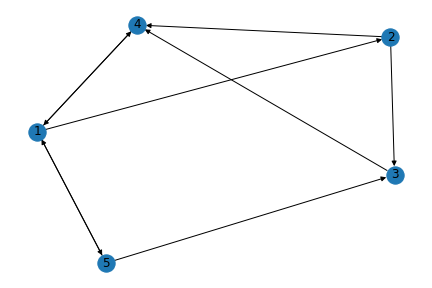
\includegraphics[scale=0.7]{images/redes-1-grafo-exemplo.png}
 \fautor
\end{figure}

A figura \ref{fig:redes1:grafo-exemplo} representa um grafo que pode ser representado pela matriz:

\begin{equation}
A = \begin{bmatrix}
0 & 1 & 0 & 1 & 1 \\
0 & 0 & 1 & 1 & 0 \\
0 & 0 & 0 & 1 & 0 \\
1 & 0 & 0 & 0 & 0 \\
1 & 0 & 1 & 0 & 0 \\
\end{bmatrix}
\end{equation}

\subsection{Métricas}
\label{section:metodologia:redes:metricas}

A seguir são descritas algumas métricas de caracterização de redes e vértices usados no decorrer do trabalho.

\subsubsection{Grau}
\label{section:metodologia:redes:metricas:grau}

O \textbf{grau} de um vértice, também denotado por $<k>$, é o número de arestas adjacentes a este vértice. No caso de grafos direcionados, o número de arestas que partem de um determinado vértice é chamado \textbf{grau de saída}, enquano o número de arestas que chegam a um determinado vértice é chamado \textbf{grau de entrada}. Em um grafo ponderado, pode-se calcular também o \textbf{grau ponderado} de um vértice através da soma dos pesos de cada aresta conectada aquele vértice.

O \textbf{grau médio} de uma rede é definido como:

\begin{equation}
    <k>_G = \frac{1}{n} \sum_{i=0}^{n} <k>_i
\end{equation}

Enquanto o \textbf{grau médio ponderado} é definido da mesma forma mas através da soma do grau ponderado de cada vértice.

A \textbf{densidade} de um grafo indica a razão de arestas que existem em relação a todas as conexões possíveis. Para grafos não-direcionados ela é definida como:

\begin{equation}
    d = \frac{2m}{n(n-1)}
\end{equation}

Enquanto para grafos direcionados ela é definida como:

\begin{equation}
    d = \frac{m}{n(n-1)}    
\end{equation}

\subsubsection{Caminhos mínimos}
\label{section:metodologia:redes:metricas:caminhos-minimos}

Um \textbf{caminho} é definido como uma sequência de vértices $v_i, v_{i+1}, ..., v_k$ de forma que exista uma aresta $e_{ij}$ que conecta cada vértice $v_i$ ao vértice $v_{i+1}$. A distância percorrida por um caminho é dado pela quantidade de arestas que o compõe. O \textbf{caminho mínimo} entre dois vértices é o caminho de menor quantidade de arestas que leva de um vértice a outro. A \textbf{distância} entre dois vértices é dada pela distância percorrida pelo caminho mínimo entre elas.

Em grafos ponderados, a \textbf{distância ponderada} é dada pela soma de todos os pesos $w_{ij}$ pertencentes às arestas de um caminho. O \textbf{caminho mínimo ponderado} é definido como o caminho de menor valor que leva de um vértice a outro.

Um grafo é chamado \textbf{conexo} se existe um caminho entre qualquer par de vértices, e \textbf{desconexo} caso contrário. Uma \textbf{componente conexa} é um subgrafo conexo maximal, isto é, que um subgrafo que não está estritamente contido em outros subgrafos conexos. A \textbf{maior componente conexa} é a componente conexa de um grafo que tenha o maior número de vértices em relação às demais. Para as formulações a seguir vamos supor que as medidas são aplicadas sobre um grafo conexo.

\subsubsection{Excentricidade}
\label{section:metodologia:redes:metricas:excentricidade}

A \textbf{excentricidade} de um vértice é dado pela distância máxima entre este vértice e todos os outros. O \textbf{diâmetro} de uma rede é dado pela excentricidade máxima dentre todos os vértices da rede, e o \textbf{raio} é dado pela excentricidade mínima.

\subsubsection{Transitividade}
\label{section:metodologia:redes:metricas:transitividade}

Essa métrica foi descrita por \citeonline{luce1949method}, e posteriormente nomeada e aprofundada por \citeonline{wasserman1994social}, e é definida da seguinte forma: uma \textbf{tríade} é definida por duas arestas que compartilham o mesmo vértice. Um \textbf{triângulo} é definido como três vértices que são conectados entre si. A \textbf{transitividade} de um grafo é definida como:

\begin{equation}
    T = 3 \frac{\#triades}{\#triangulos}
\end{equation}

onde $\#triades$ mede a quantidade de tríades em um grafo, e $\#triangulos$ a quantidade de triângulos.

A transitividade também é conhecida como \textbf{coeficiente de agrupamento global}, pois indica o quão agrupados são os vértices de uma rede. Da mesma forma, proposto por \citeonline{watts1998collective}, defini-se o \textbf{coeficiente de agrupamento local} de um vértice $i$ como:

\begin{equation}
    c_i = \frac{2 T_i}{<k>_i (<k>_i - 1)}
\end{equation}

Para grafos ponderados, usa-se a média geométrica dos pesos das arestas:

\begin{equation}
    c_i = \frac{2 T_i}{<k>_i (<k>_i - 1)} \sum_{jk} (w_{ij} w_{ik} w_{jk})^{\frac{1}{3}}
\end{equation}

Neste caso, é comum que seja feita a normalização dos pesos dos vértices em relação ao peso máximo da rede.

\subsubsection{Assortatividade}
\label{section:metodologia:redes:metricas:assortatividade}

A \textbf{assortatividade} é uma métrica de correlação entre as características dos vértices de uma rede. Ela é descrita por \citeonline{newman2003mixing} e é calculada a partir de uma matriz $e$ em que cada elemento $e_{ij}$ representa a fração das arestas da rede que conectam um vértice do tipo $i$ a um vértice do tipo $j$. Então são definidos:

\begin{equation}
    a_i = \sum_j e_{ij}, \: b_j = \sum_i e_{ij}
\end{equation}

O coeficiente de assortatividade é então definido da seguinte maneira:

\begin{equation}
    r = \frac{\sum\limits_i e_{ii} - \sum\limits_i a_i b_i}{1 - \sum\limits_i a_i b_i}
\end{equation}

Quando $r=1$, a rede é totalmente \textbf{assortativa} e seus vértices tendem a se conectar apenas a vértices semelhantes, enquanto $r=-1$ representa uma rede totalmente \textbf{disassortativa} onde os vértices se conectam apenas à vértices diferentes. Por fim, $r=0$ indica uma rede \textbf{não-assortativa} onde os vértices não tem uma preferência definida.

A assortatividade pode ser utilizada para medir a correlação entre qualquer atributo relacionado aos vértices e de uma rede. A \textbf{assortatividade de grau}, por exemplo, é comumente usada para medir a preferência de vértices mais conectados, chamados \textit{hubs}, de se conectar com vértices menos conectados, e vice-versa. Enquanto cada vértice pode ter um atributo relacionado, por exemplo o sexo de uma pessoa, e podemos então medir a preferência de homens e mulheres de se conectarem a pessoas de determinado sexo em uma rede social.

\subsubsection{Centralidade}
\label{section:metodologia:redes:metricas:centralidade}

A centralidade pode ser intuitivamente definida como a medida de importância de um vértice em uma rede. Quanto mais \textit{central} é um véritce, maior a importância dele para a rede. Existem várias formas de se calcular a centralidade, sob diversos pontos de vista, os quais apresentaremos a seguir.

A primeira forma de calcular centralidade é utilizando a \textbf{centralidade de grau}. A centralidade de grau $c_i$ de um vértice $i$ é calculada pela fração dos vértices de uma redes que estão conectada ao um vértice $i$:

\begin{equation}
    c_i = \frac{<k>_i}{n}
\end{equation}

Ou seja, essa medida é análoga ao grau de um vértice mas normalizado pela quantidade de vértices da rede.

\citeonline{freeman1979centrality} define outra métrica de centralidade, a \textbf{centralidade de proximidade}. Ela é definida como a distância média entre um vértice e todos os outros daquela rede, da seguinte forma:

\begin{equation}
    c_i = \frac{n-1}{\sum\limits_{j=0}^{n} d(i,j)}
\end{equation}

onde $d(i,j)$ indica a distância entre os vértices $i$ e $j$.

Uma variação da centralidade de proximidade é a \textbf{centralidade de informação}, proposta por \citeonline{stephenson1989rethinking}, que ao invés de utilizar a distância como medida usa a distância resistiva, uma medida derivada de sistemas elétricos, para representar o fluxo de informação entre dois vértices.

Outra medida relacionada a caminhos mínimos, a \textbf{centralidade de intermediação} também proposta por \citeonline{freeman1977set} mede a participação de um vértice em relação a todos os caminhos mínimos entre quaisquer vértices da rede. Dessa forma, definimos a centralidade de intermediação da seguinte forma:

\begin{equation}
    c_i = \sum_{j=0,k=0}^{n} \frac{\sigma(j,k|i)}{\sigma(j,k)}
\end{equation}

sendo que $\sigma(j,k)$ denota a quantidade de caminhos mínimos entre $j$ e $k$, e $\sigma(j,k|i)$ denota quantos desses caminhos passam por $k$. Tal medida pode ou não usar a formulação ponderada para caminhos mínimos.

A \textbf{centralidade de autovalor}. proposta por \citeonline{bonacich1987power}, usa uma formulação matricial para a sua formulação. Através de uma formulação recursiva, podemos definir a centralidade de um vértice através da centralidade de seus vizinhos usando uma matriz de adjacências $A_{ij}$:

\begin{equation}
    c_i = \frac{1}{\lambda} \sum\limits_{j \in adj(i)} a_{ij} c_j
\end{equation}

sendo $\lambda$ uma constante e $adj(i)$ se refere a lista de vizinhos de $i$. A centralidade de um vértice é então, de forma simplificada, a soma da centralidade de seus vizinhos. Ao rearranjar essa formulação, obtemos:

\begin{equation}
    A x = \lambda x
\end{equation}

também chamada de equação de autovalores, uma equação comum na Álgebra Linear e que possui diferentes métodos de solução através de métodos iterativos, como o Método das Potências de \citeonline{mises1929praktische}.

Outro método baseado na centralidade de autovalores é o algoritmo \textbf{PageRank}, proposto pelos fundadores da Google \citeonline{page1999pagerank}, que utiliza uma formulação análoga mas considerando a direção das arestas, recebendo maior centralidade o vértice que possui arestas que partem de vértices também de alta centralidade.

\section{Análise de Componentes Principais}
\label{section:metodologia:pca}

Proposto por \citeonline{pearson1901liii}, a Análise de Componentes Principais, também chamada PCA do inglês Principal Components Analysis, é uma ferramenta comum de análise exploratória de dados. O PCA é definido como uma transformação linear ortogonal aplicada a uma matriz para que os dados sejam projetados em um novo sistemas de coordenadas de forma que as coordenadas estejam ordenadas refletindo a variância de cada coordenada.

Intuitivamente, o objetivo com PCA é encontrar uma base que diminua a redundância entre um conjunto de variáveis analisadas. Uma medida de redundância é a correlação entre duas variáveis, se eles são totalmente correlacionadas então existe muita redundância no conjunto de variáveis e podemos reduzir a quantidade de variáveis sem perda de informação, por exemplo.

Aplicando esse método sobre uma matriz $X_{nxm}$ com $m$ variáveis que descrevem $n$ experimentos, obtemos uma matriz de autovetores $A_{nxm}$, e um vetor de autovalores $V_{mx1}$. Cada componente do vetor de autovalores indicará a quantidade de variância que a aquela componente principal explica. Intuitivamente, se normalizarmos o vetor de autovalores, podemos obter o percentual de informação que cada componente contém em relação ao conjunto de dados inicial, ou seja, o primeiro componente do vetor indicará a variância explicada pela primeira componente, a segunda indica a variância da segunda componente, e assim por diante. A matriz de autovetores indica a influência de cada variável em relação a cada componente, ou seja, a primeira linha desta matriz indicará a direção da transformação aplicada sobre cada variável para a primeira componente, e quanto maior a magnitude dessa direção, maior a influência dessa variável sobre aquela componente.

A PCA pode ser utilizada para diminuição de dimensionalidade, uma vez que selecionando as duas primeiras componentes principais podemos, por exemplo, projetar os dados iniciais em um espaço de duas dimensões, e então ter uma visualização dos dados em um espaço cartesiano de forma que sabemos quanto da informação contida no conjunto de dados inicial está explicada ali. Isso é particularmente útil para observar o espalhamento de dados para problemas de classificação.

\section{Classificadores}
\label{section:metodologia:classificadores}

Nesta seção, serão apresentados alguns conceitos e métodos de classificação utilizados no decorrer desta dissertação.

\subsection{Conceitos}
\label{section:metodologia:classificadores:conceitos}

\citeonline{vapnik1999overview} nos dá uma visão geral da Teoria do Aprendizado Estatístico, um campo introduzido em 1960, com uma formulação de como ocorre o aprendizado. Ele modela o problema do aprendizado da seguinte forma: são dados três componentes:

\begin{enumerate}
    \item Uma distribuição desconhecida $P(x)$
    \item Um supervisor capaz de produzir um vetor $y$ a partir de uma distribuição também desconhecida $P(y|x)$
    \item Uma máquina de aprendizado capaz de implementar um conjunto de funções $f(x,\alpha)$
\end{enumerate}

O aprendizado é descrito como um problema de minimização do risco, definido como:

\begin{equation}
    R(\alpha) = \int L(y,f(x,\alpha)) dP(x,y)
\end{equation}

Queremos escolher uma função $f(x,\alpha)$ de forma que o risco seja o menor possível. De forma intuitiva, queremos construir algoritmos que sejam capazes de rotular dados de forma eficiente. 

Geralmente, se divide o problema do aprendizado em \textbf{classificação}, quando os rótulos são discretos, e \textbf{regressão}, quando são contínuos.

Uma vez aplicado um algoritmo de classificação, existem uma série de métricas para avaliarmos se houve sucesso ou não na tarefa. Para um problema binário, onde queremos rotular um conjunto de entidades em Positivos e Negativos, podemos construir uma \textbf{matriz de confusão} como ilustrado no quadro \ref{quadro:matriz_de_confusão}.

\begin{quadro}[htb]
\caption{Matriz de confusão}
\label{quadro:matriz_de_confusão}
\centering
\begin{tabular}{c|c}
Verdadeiros Negativos (VN) & Falsos Positivos (FN) \\ \hline
Falsos Negativos (FP) & Verdadeiros Positivos (VP) \\
\end{tabular}
\end{quadro}

Ou seja, cada linha representa o rótulo esperado e cada coluna representa o rótulo predito pelo classificador. O rótulo predito pode ser Verdadeiro ou Falso, se o classificador tiver acertado ou não.

A primeira métrica usada para a análise de classificadores é a \textbf{acurácia}, que mede quantas predições o classificador acertou em relação ao total de amostras:

\begin{equation}
    A = \frac{VP+VN}{Total}
\end{equation}

Essa métrica nos diz quanto um determinado classificador acerta em relação ao total, mas isso nem sempre é suficiente, principalmente em conjuntos de dados desbalanceados.

A \textbf{precisão} indica quantos Positivos eram de fato Positivos quando foram classificados dessa forma:

\begin{equation}
    P = \frac{VP}{VP+FP}
\end{equation}

Outras duas métricas são importantes, a \textbf{sensibilidade}, também chamada \textit{recall}, que indica quantos de todos os casos Positivos foram efetivamente rotulados corretamente:

\begin{equation}
    S = \frac{VP}{VP+FN}
\end{equation}

E a \textbf{especificidade}, que faz o mesmo para Negativos:

\begin{equation}
    E = \frac{VN}{VN+FP}
\end{equation}

Para ponderar especificidade e sensibilidade, existe a medida \textbf{F1-score}, que é a média harmônica entre precisão e sensibilidade:

\begin{equation}
    F = 2\frac{P*S}{P+S}
\end{equation}

Outro meio de avaliar um classificador, usando um método visual, é a curva ROC, do inglês Receiver Operating Characteristic, ou em tradução lívre Característica de Operação do Receptor. Essa curva representa um gráfico da especificidade de um algoritmo em relação a sua sensibilidade, ilustrado na Figura~\ref{fig:metodologia:curva-roc-exemplo}.

\begin{figure}[htb]
	\centering
    \caption{Exemplo de Curva ROC}
    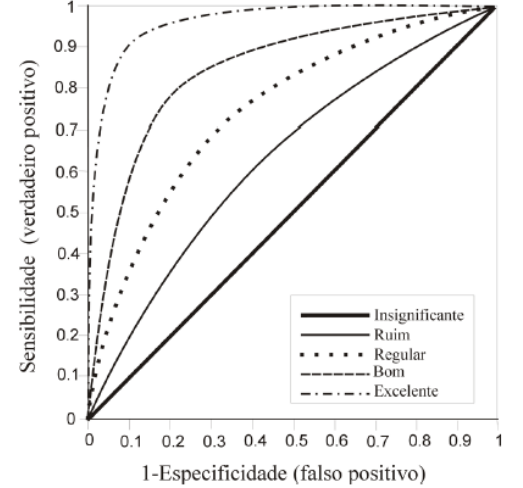
\includegraphics[scale=0.5]{images/curva-roc-exemplo.png}
    \label{fig:metodologia:curva-roc-exemplo}
    \fdireta[p.06]{souza2008analise}
\end{figure}

Para a validação da performance de um classificador sobre um conjunto de dados são utilizadas também uma série de técnicas. A maior parte dessas técnicas utiliza uma divisão do conjunto de dados em conjunto de treino e outro conjunto de testes. O primeiro é utilizado pelo classificador para que este ajuste seus parâmetros, e posteriormente este classificador é aplicado ao conjunto de validação e então são observados os resultados.

Um método comum para conjuntos de dados pequenos é o \textbf{leave-one-out}, em tradução livre \textit{deixe um fora}. Neste método, para um conjunto de dados com $N$ amostrar, são feitos $N$ testes onde a cada iteração uma amostra é escolhida como teste e todo o restante do conjunto de dados é utilizado como conjunto de treino. Essa é uma das formas mais fortes de validação de um algoritmo, uma vez que toda informação é usada para classificação.

Outra técnica comumente usada, mas em conjuntos de dados maiores, chama-se \textbf{k-fold}, ou \textit{k-dobras}. Nela, o conjunto de dados é dividido em $k$ subconjuntos mutualmente exclusivos, e a cada iteração $k-1$ subconjuntos são utilizados para treinamento e o subconjunto restante é utilizado para validação. Essa técnica também possui sua versão estratificada que mantém a proporção de classes do conjunto inicial.

Algo importante de se observar em todo classificador é o dilema viés-variância. O \textbf{viés} de um classificador é a tendência dele de fazer suposições erradas sobre o conjunto de dados. Um alto viés ira causar \textbf{underfitting}, isto é, o classificador será incapaz de prever características nos dados necessárias para rotular corretamente os dados. Por outro lado, viés é algo necessário para que o classificador seja objetivo.

A \textbf{variância} se refere à capacidade de um algoritmo de lidar com diferentes características em um conjunto de dados. Um algoritmo com alta sensibilidade à variância irá utilizar cada pequena diferença nos dados para rotular os dados, não conseguindo alcançar o que é chamado de \textbf{generalização}. A generalização é a capacidade de um algoritmo de classificação de rotular corretamente os dados ignorando ruídos nos dados, evitando \textbf{overfitting}, isto é evitando que o classificador seja demasiadamente influenciado pelo conjunto de treino.

\begin{figure}[htb]
	\centering
    \caption{O dilema viés-variância}
    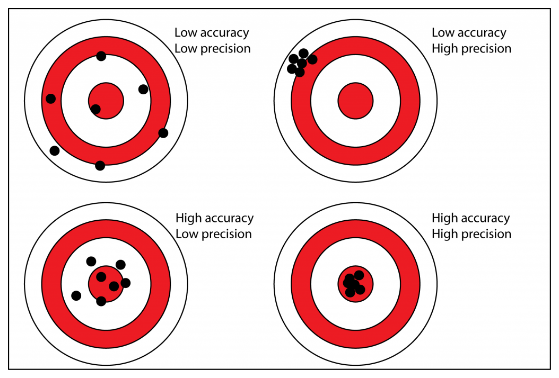
\includegraphics[scale=0.5]{images/variancia-vies.png}
    \label{fig:variancia-vies}
    \fdireta[p.01]{variancia2019vies}
\end{figure}

A seguir, utilizamos alguns classificadores utilizados neste trabalho.

\subsection{K-Nearest Neighbors}
\label{section:metodologia:classificadores:knn}

O primeiro algoritmo aqui citado é o K-Neares Neighbors, ou em tradução livre K-Vizinhos mais próximos. Este classificador, desenvolvido por \citeonline{fix1951discriminatory}, é um dos mais comumente utilizados como referência dada usa simplicidade.

Este algoritmo funciona através do cálculo da distância entre pontos no espaço multidimensional. Para classificar cada amostra, o algoritmo calcula quais são as $k$ amostras mais próximas e faz uma votação entre elas para decidir qual será o rótulo predito para a amostra sendo testada. O rótulo mais comum dentre os vizinhos de uma amostra indicará o rótulo desta amostra.

Este é um método de baixa complexidade computacional, uma vez que o parâmetro $k$ é escolhido e funciona bem para problemas onde há uma boa separação espacial das classes.

\subsection{Random Forest}
\label{section:metodologia:classificadores:random-forest}

O classificador random forest, ou florestas aleatórias, é um classificador \textit{ensemble}, isto é, um classificador que se utiliza de diversos classificadores. O algoritmo se utiliza de árvores aleatórias de decisão, propostas por \citeonline{ho1995random} a partir do trabalho de discriminzação estatística proposta por \citeonline{kleinberg1990stochastic}.

Uma árvore de decisão é uma estrutura de decisão construída a partir do conjunto de treino. Nela, cada folha representará um estado, e cada vértice do topo até as folhas representará uma variável e condições relacionadas a essa variável. Para classificar um teste, percorre-se essa árvore desde o topo, e para cada nó verificam-se as condições necessárias para seguir para um dos vértices-filhos até que se chegue a uma folha.

Uma árvore de decisão pode ser construída de várias formas, geralmente utilizando uma abordagem \textit{top-down}, onde a cada nova amostra de treino, a árvore é percorrida e é calculado o ganho de informação com uma nova divisão da árvore. Existem diversas métricas de ganho de informação, como por exemplo o coeficiente de gini ou entropia. De forma intuitiva, uma árvore de decisão divide o espaço em diversas regiões retangulares delimitadas pelas condições para divisão de cada variável.

O algoritmo de florestas aleatórias cria então diversas árvores de decisão e ao classificar uma amostra de teste faz uma eleição dentre elas para então rotular o dado. Este algoritmo é eficiente em situações onde há um bom espalhamento dos dados e é particularmente sensível a \textit{overfitting}, sendo computacionalmente eficiente.

\subsection{Regressão Logística}
\label{section:metodologia:classificadores:regressao-logistica}

Segundo \citeonline{cramer2002origins}, a regressão logística é produto de diversos trabalhos nos séculos XVIII e XIX. A regressão logística é usada hoje como técnica de classificação que aplica uma regressão sobre a função logística, também chamada sigmóide \cite{logistic2017regression}:

\begin{equation}
    \sigma (x) = \frac{1}{1+e^{-x}}
\end{equation}

O que essa técnica faz é minimizar a chamada entropia cruzada, aqui denotada por:

\begin{equation}
    E = \begin{cases}
        -log(\hat{x}), \: se \: x=1
        -log(1-\hat{x}), \: se \: x=0
        \end{cases}
\end{equation}

onde $x$ é o rótulo real e $\hat{x}$ o rótulo previsto. Veja que se $x=1$ e $\hat{x}=0$, então $E$ será infinito, o que também ocorre se $x=0$ e $\hat{x}=1$, ou seja, estamos penalizando erros de classificação com essa modelagem. Podemos reescrever o nosso objetivo então como:

\begin{equation}
    E = \sum -x log(\hat{x})-(1-x)log(1-\hat{x})
\end{equation}

Minimizando essa função, obteremos uma série de parâmetros que podem ser utilizados para predizer um valor $\hat{x}$ para uma amostra, que irá variar entre 0 e 1, que são interpretadas como a chance dessa amostra pertencer a uma classe ou outra.

Esse método é particularmente eficiente em situações onde já diferenças consideráveis entre as classes, seja desbalanceamento ou diferentes variâncias, sendo bastante útil.

\subsection{SVC}
\label{section:metodologia:classificadores:svc}

Por fim, o último método aqui utilizado é \textit{Support Vector Classifier}, ou Classificadores de Vetores de Suporte. As Máquinas de Vetores de Suporte foram propostas a partir da Teoria do Aprendizado Estatístico por \citeonline{vapnik1963pattern}.

Intuitivamente, as máquinas de vetores de suporte encontram o superplano que melhor divide os dados de um conjunto de dados maximizando a distância entre este superplano e cada uma das classes. Ou seja, dada uma lista $(x_1,y_1),...,(x_n,y_n)$ onde $x_i$ representa um ponto no espaço, e cada $y_i$ representa uma classe binária.

Usando a formulação linear, queremos encontrar o hiperplano que maximize a distância entre ele e o conjunto de pontos $x_1,...,x_n$. O vetor normal ao hiperplano pode ser escrito como:

\begin{equation}
    w^T x-b=0
\end{equation}

Se o nosso conjunto de dados for linearmente separável, podemos então definir outros dois hiperplanos: $w^T x-b=1$ e $w^T x-b=-1$ que indicam a borda de cada uma das classes no conjunto de dados. Isto é, qualquer ponto localizado em $w^T x-b \geq 1$ terá classe 1, e qualquer ponto localizado em $w^T x-b \leq -1$ terá classe -1.

Sendo assim, esse classificador pode ser descrito pelo problema de otimização de minimização da seguinte função:

\begin{equation}
    y(w^T x-b) \geq 1
\end{equation}

Esse classificador é bastante eficiente caso o conjunto de dados seja separável. Existem outras funções que podem ser utilizadas para separar os dados, como sigmóide e polinômios.

